%%%%%%%% ICML 2023 EXAMPLE LATEX SUBMISSION FILE %%%%%%%%%%%%%%%%%

\documentclass{article}

% Recommended, but optional, packages for figures and better typesetting:
\usepackage{microtype}
\usepackage{graphicx}
\usepackage{subfigure}
\usepackage{booktabs} % for professional tables

% hyperref makes hyperlinks in the resulting PDF.
% If your build breaks (sometimes temporarily if a hyperlink spans a page)
% please comment out the following usepackage line and replace
% \usepackage{icml2023} with \usepackage[nohyperref]{icml2023} above.
\usepackage{hyperref}


% Attempt to make hyperref and algorithmic work together better:
\newcommand{\theHalgorithm}{\arabic{algorithm}}

% Use the following line for the initial blind version submitted for review:
\usepackage{icml2023}

% If accepted, instead use the following line for the camera-ready submission:
% \usepackage[accepted]{icml2023}

% For theorems and such
\usepackage{amsmath}
\usepackage{amssymb}
\usepackage{mathtools}
\usepackage{amsthm}

% if you use cleveref..
\usepackage[capitalize,noabbrev]{cleveref}

%%%%%%%%%%%%%%%%%%%%%%%%%%%%%%%%
% THEOREMS
%%%%%%%%%%%%%%%%%%%%%%%%%%%%%%%%
\theoremstyle{plain}
\newtheorem{theorem}{Theorem}[section]
\newtheorem{proposition}[theorem]{Proposition}
\newtheorem{lemma}[theorem]{Lemma}
\newtheorem{corollary}[theorem]{Corollary}
\theoremstyle{definition}
\newtheorem{definition}[theorem]{Definition}
\newtheorem{assumption}[theorem]{Assumption}
\theoremstyle{remark}
\newtheorem{remark}[theorem]{Remark}

% Todonotes is useful during development; simply uncomment the next line
%    and comment out the line below the next line to turn off comments
%\usepackage[disable,textsize=tiny]{todonotes}
\usepackage[textsize=tiny]{todonotes}

% math shih
\newcommand{\setof}[1]{\left\{{#1}\right\}}
\newcommand{\given}{\,|\,}
\newcommand{\lss}{{\small{LSS}}\xspace}

\newcommand{\Om}{\Omega_{\rm m}} 
\newcommand{\Ob}{\Omega_{\rm b}} 
\newcommand{\OL}{\Omega_\Lambda}
\newcommand{\smnu}{M_\nu}
\newcommand{\sig}{\sigma_8} 
\newcommand{\mmin}{M_{\rm min}}
\newcommand{\BOk}{\widehat{B}_0} 
\newcommand{\hmpc}{\,h/\mathrm{Mpc}}
\newcommand{\bfi}[1]{\textbf{\textit{#1}}}
\newcommand{\parti}[1]{\frac{\partial #1}{\partial \theta_i}}
\newcommand{\partj}[1]{\frac{\partial #1}{\partial \theta_j}}
\newcommand{\mpc}{{\rm Mpc}}
\newcommand{\eg}{\emph{e.g.}}
\newcommand{\ie}{\emph{i.e.}}



% The \icmltitle you define below is probably too long as a header.
% Therefore, a short form for the running title is supplied here:
\icmltitlerunning{Cosmology with Only the Photometry of Galaxies}

\begin{document}

\twocolumn[
\icmltitle{Cosmology with Only the Photometry of Galaxies}

% It is OKAY to include author information, even for blind
% submissions: the style file will automatically remove it for you
% unless you've provided the [accepted] option to the icml2023
% package.

% List of affiliations: The first argument should be a (short)
% identifier you will use later to specify author affiliations
% Academic affiliations should list Department, University, City, Region, Country
% Industry affiliations should list Company, City, Region, Country

% You can specify symbols, otherwise they are numbered in order.
% Ideally, you should not use this facility. Affiliations will be numbered
% in order of appearance and this is the preferred way.
\icmlsetsymbol{equal}{*}

\begin{icmlauthorlist}
\icmlauthor{ChangHoon Hahn}{0}
\icmlauthor{Francisco Villaescusa-Navarro}{1}
\end{icmlauthorlist}

\icmlaffiliation{0}{Department of Astrophysical Sciences, Princeton University, Peyton Hall, Princeton NJ 08544, USA}

\icmlcorrespondingauthor{Firstname1 Lastname1}{first1.last1@xxx.edu}
\icmlcorrespondingauthor{Firstname2 Lastname2}{first2.last2@www.uk}

% You may provide any keywords that you
% find helpful for describing your paper; these are used to populate
% the "keywords" metadata in the PDF but will not be shown in the document
\icmlkeywords{Machine Learning, ICML}

\vskip 0.3in
]

% this must go after the closing bracket ] following \twocolumn[ ...

% This command actually creates the footnote in the first column
% listing the affiliations and the copyright notice.
% The command takes one argument, which is text to display at the start of the footnote.
% The \icmlEqualContribution command is standard text for equal contribution.
% Remove it (just {}) if you do not need this facility.

%\printAffiliationsAndNotice{}  % leave blank if no need to mention equal contribution
\printAffiliationsAndNotice{\icmlEqualContribution} % otherwise use the standard text.

\begin{abstract}
    We present the first cosmological constraints from only the observed
    photometry of galaxies. 
    \cite{villaesucsa-navarro2022} recently demonstrated that a galaxy's 
    internal physical properties contain a significant amount of cosmological
    information.
    These physical properties, however, cannot be directly measured from
    observations. 
    In this work, we present how we can go beyond theoretical demonstrations to
    infer cosmological constraints from actual galaxy observables (\emph{e.g.}
    optical photometry) using neural density estimation and the CAMELS suite of 
    hydrodynamical simulations. 
    We find that the cosmological information in the photometry of a single
    galaxy is limited.
    However, we can combine the constraining power of photometry from many
    galaxies using hierarchical population inference and place significant
    cosmological constraints.
    With the observed photometry of $\sim$15,000 NASA-Sloan Atlas galaxies, we 
    constrain $\Omega_m=0.290^{+0.077}_{-0.088}$ and
    $\sigma_8=0.793^{+0.098}_{-0.092}$. 
\end{abstract}

% --- intro ---  
\section{Introduction} \label{sec:intro} 
In recent work, Villaescusa-Navarro~et~al.~\yrcite{villaescusa-navarro2022}
showed that it is possible to place cosmological constraints from only the
internal properties of a single galaxy.
They used galaxies from 2,000 state-of-the-art hydrodynamical simulations with
different cosmologies and astrophysical models from
CAMELS~\citep{villaescusa-navarro2021, villaescusa-navarro2022a} to train
moment networks~\citep{jeffrey2020a} that predict cosmological parameters from
galaxy properties. 
With only a handful of galaxy properties, including stellar mass ($M_*$),
stellar metallicity ($Z_*$), and maximum circular velocity ($V_{\rm max}$),
they were able to constrain $\Omega_m$ to 10\% precision with a single galaxy.
They found similar constraining power for galaxies simulated using the subgrid
physics models of the IllustrisTNG~\citep{pillepich2018, weinberger2018} and
SIMBA~\citep{dave2019}. 
Since then, follow-up works have found consistent results for other
hydrodynamicl models: \citep{echeverri2023}. 


According to Villaescusa-Navarro~et~al.~\yrcite{villaescusa-navarro2021}, the
cosmological information is derived from the imprint of $\Omega_m$ on the dark
matter content of galaxies that affects galaxy properties in a distinct way
than astrophysical processes.
Also, since $\Omega_b$ is fixed in CAMELS, which is justified by the tight
constraints from Big Bang Nucleosynthesis, the galaxy properties are
effectively measuring the baryon fraction, $\Omega_b/\Omega_m$.
For instance, $V_{\rm max}$ measures the depth of the total matter
gravitational potential while other properties like $M_*$ and $Z_*$ measures
the mass in baryons so together they can constrain the ratio
$\Omega_b/\Omega_m$.
In fact, a similar approach was used three deacdes ago in 
White et al. \yrcite{white1993} to constrain $\Omega_b/\Omega_m$  using galaxy
clusters. 

Despite the promising signs that they may be useful cosmological probes, galaxy
properties themselves are {\em not} actual observable.
They are derived quantities that are typically inferred from photometry or
spectra of galaxies and require modeling the spectral energy distribution
(SED) or emission lines~\citep{conroy2013}.
In this work, we go beyond the theoretical considerations of previous works and
infer cosmological parameters from actual galaxy observables --- optical  
photometry.  
We leverage a simulation-based inference method that employs neural density
estimation to estimate the posterior of cosmological parameters given galaxy
photometry, similar to the approach of \cite{hahn2022a}. 
Furthermore, since we expect a limited amount of cosmological information from
the photometry of a single galaxy, we present a hierarhical population
inference approach for inferring the posterior of cosmological parameters
from the photometry of multiple galaxies. 
Lastly, we present the cosmological constraints derived from applying this
approach to the photometry of $\sim$15,000 SDSS galaxies from the NASA-Sloan
Atlas (Sec.~\ref{sec:nsa}). 

% --- data ---  
\section{Data} \label{sec:data}
\subsection{NASA-Sloan Atlas}  \label{sec:nsa}
For our observations, we use galaxy photometry from the NASA-Sloan
Atlas\footnote{\url{http://www.nsatlas.org/}} (hereafter NSA).
The NSA provides photometry of $z < 0.05$ galaxies observed by the Sloan
Digital Sky Survey Data Release 8~\citep[SDSS;][]{aihara2011} with
improved background subtraction~\citep{blanton2011}. 
In particular, we use optical $g$, $r$, $i$, $z$ band absoluate magnitudes
derived using {\sc kcorrect}~\citep{blanton2007}, assuming a
\cite{chabrier2003} initial mass function. 
In Fig.~\ref{fig:nsa}, we present the $(g - r) - M_r$ color-magnitude
distribution of $\sim120,000$ NSA galaxies (black), which reveals the modes 
that correspond to blue star-forming and red quiescent galaxies. 

Among the full NSA sample, we focus on luminous galaxies with 
$-18 > M_r > -22$.
We exclude galaxies brighter than $M_r > -22$ since our simulated galaxy sample
does not include a large number of the most luminous galaxies. 
In addition, we only select galaxies with precisely measured photometry: 
magnitude uncertainties below $\sigma_g, \sigma_r, \sigma_i < 0.022$ and 
$\sigma_z < 0.04$. 
Lastly, we impose the color cuts to exclude galaxies within the
central 68 percentile of the $g-r$, $g-i$, $g-z$, $r-i$, $r-z$, $i-z$ color
distributions.
The color cuts remove NSA galaxies that potentially have observational
artifacts or problematic photometry.
They also ensure that the NSA galaxies are within the photometric distribution
(\ie~support) of the simulated galaxies used in this work.
We mark the 95$^{th}$ percentile contour of our NSA subsample in
Fig.~\ref{fig:nsa} (black dot-dashed).
In total, we use 14,736 NSA galaxies.


\begin{figure}[ht]
\vskip 0.2in
\begin{center}
    \centerline{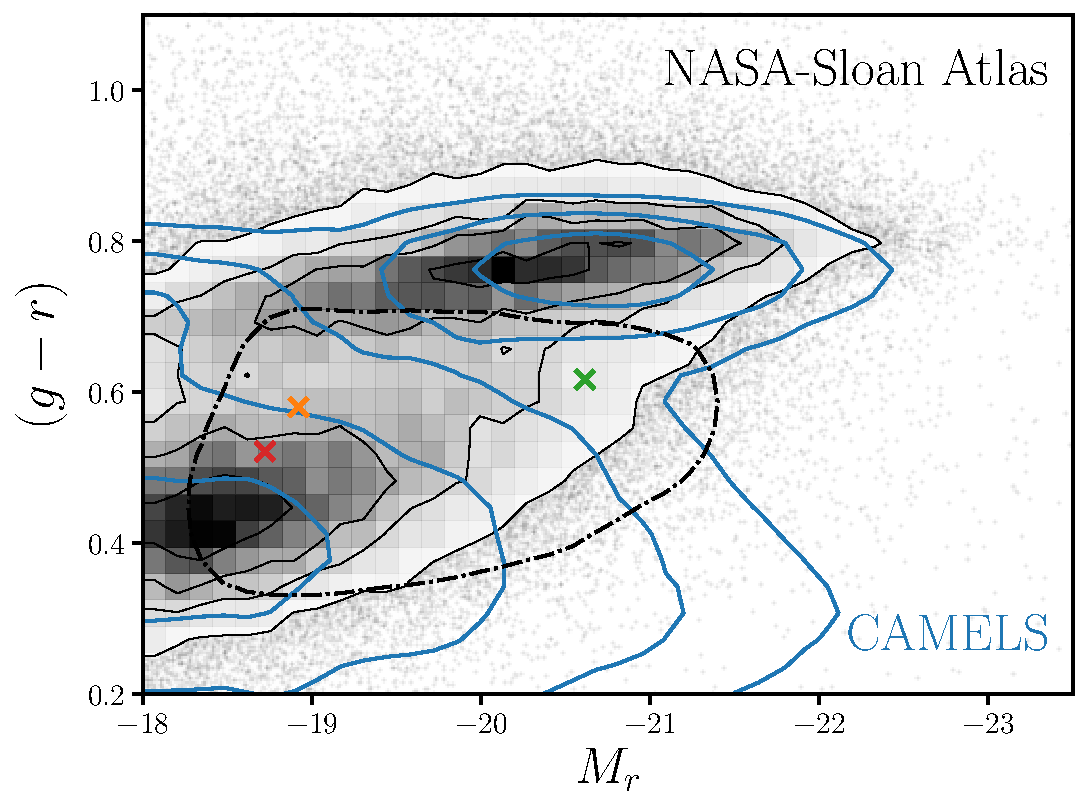
\includegraphics[width=\columnwidth]{figs/nsa.pdf}}
    \caption{Color-magnitude distrubtion, $(g-r) - M_r$, of observed galaxies
    from the NSA (black) and simulated galaxies from CAMELS-TNG (blue). 
    The distribution reveals the bimodality distribution of blue star-forming
    and red quiescent galaxies. 
    Overall, the distributions of NSA and CAMELS-TNG galaxies are in good
    agreement. 
    The distribution for CAMELS-TNG is significantly broader since its simulated
    galaxies are generated using a wide range of cosmological and baryonic
    feedback parameters.
    }\label{fig:nsa}
\end{center}
\vskip -0.2in
\end{figure}

\subsection{Forward Model: CAMELS} \label{sec:sims} 
In this work, we also use simulated galaxies from the Cosmology and
Astrophysics with MachinE Learning
Simulations~\citep[CAMELS;]{villaescusa-navarro2021, villaescusa-navarro2022a},
a suite of hydrodynamical simulations constructed over a wide
range of cosmological and hydrodynamical parameters.
In particular, we use the 1,000 hydrodynamical simulations (CAMELS-TNG)
constructed using the subrid physics model of the state-of-the-art
IllustrisTNG~\citep{nelson2019}. 
The simulations are generated with different cosmoloigcal parameters,
$\Omega = \{\Omega_m, \sigma_8\}$, and baryonic feedback parameters, 
$\mathcal{B} = \{A_{\rm SN1}, A_{\rm SN2}, A_{\rm AGN1}, A_{\rm AGN2}\}$,
arranged in a latin hypercube. 
$A_{\rm SN1}$ and $A_{\rm SN2}$ represent the normalization factors for the 
galactic wind flux and speed; 
$A_{\rm AGN1}$ and $A_{\rm AGN2}$ represent the normalization factors for the 
energy output and specific energy of AGN feedback.
All the cosmological parameter besides $\Omega_m$ and $\sigma_8$ are fixed:
$\Omega_b = 0.049$, $h = 0.6711$, $n_s = 0.9624$, $\sum m_\nu = 0.0$eV, and 
$w = -1$.
%The CAMELS-TNG simulation all have a comoving volume of 
%(25 $h^{-1}{\rm Mpc}$)$^3$.
%They each evolve $256^3$ dark matter particles and $256^3$ fluid elements from
%$z=127$ to $z=0$ from initial conditions generated using second order
%perturbation theory. 
%Each simulation has 34 saved snapshots from $z=6$ to $z=0$. 
%Since we target $z < 0.05$ NSA galaxies, we only use the $z=0$ snapshot. 
%All the cosmological parameter besides $\Omega_m$ and $\sigma_8$ are fixed:
%$\Omega_b = 0.049$, $h = 0.6711$, $n_s = 0.9624$, $\sum m_\nu = 0.0$eV, and 
%$w = -1$.
%The SUBFIND~\citep{springel2001, dolag2009} algorithm is run on each simulation
%to identify halos and subhalos.
%SUBFIND computes physical quantities of the subhalos and the galaxies that
%resides in them. 
%For additional details on CAMELS, we refer readers to
%\cite{villaescusa-navarro2021, villaescusa-navarro2022a}.

In all 1,000 CAMELS-TNG simulations, there are $\sim$700,000 galaxies with more
than 20 star particles. 
The galaxies, however, are not evenly distributed across the simulations and
have a significant dependence on the CAMELS parameters.  
For instance, simulations constructed at higher $\Omega_m$ values have more
galaxies.  
Since the goal of this work is to conduct cosmological inference on a per
galaxy basis, we must correct for this implicit prior on the CAMELS parameters.
We do this by randomly selecting 100 galaxies from each simulation. 
This imposes a uniform prior: $p(\Omega, \mathcal{B}) = 1$. 
Thus, we use a total of 100,000 CAMELS-TNG galaxies.  

Since the goal of this work is to analyze the observed photometry of NSA
galaxies, we forward model observed photometry for the simulated galaxies. 
CAMELS-TNG already provides synthetic dust attenuated stellar photometry for
each simulated galaxy calculated using the same procedure as \cite{nelson2018}.
The unattenuated spectral energy distribution (SED) of a galaxy is computed by
combining the SEDs of every member star particle of the host subhalo. 
Each star particle SED is modeled as a single-burst simple stellar population
using stellar population synthesis (SPS) based on the recorded birth time,
metallicity, and mass. 
The SPS uses FSPS~\citep{conroy2009, conroy2010}, Padova isochrones, MILES
stellar library, and assumes a Chabrier initial mass function. 
The unattenuated galaxy SEDs are then attenuated using a dust model based on
the metal content of the neutral gas distribution in and around each
galaxy~\citep[Model C in][]{nelson2018}. 
Afterwards, the SED is convolved with SDSS $g$, $r$, $i$, $z$-band photometric
bandpasses to produce the photometry: $X_i$. 
%For additional details on the synthetic photometry, we refer readers to \cite{nelson2018}. 

Next, we add noise to the CAMELS-TNG synthetic photometry based on the measured
uncertainties, $\sigma_X$, of NSA galaxies. 
For each alaxy, we randomly sample $\sigma_{X,i}$ from the range of uncertainties 
measured in NSA. 
Afterwards, we apply the uncertainty using a Gaussian with standard deviation
$\sigma_{X,i}$: $\hat{X}_i \sim \mathcal{N}(X_i, \sigma_{X, i})$. 
Although our noise model is overly simplistic, this is not an issue in our
approach beacuse the posteriors we ultimately evaluate are conditioned on the
uncertainties~\citep{hahn2022a}. 
In Fig.~\ref{fig:nsa}, we present the color-magnitude distribution of the
forward modeled CAMELS-TNG galaxies in blue. 

% --- methods ---  
\section{Methods} \label{sec:methods} 
\subsection{Hierarchical Bayesian Inference} \label{sec:hier} 
Our goal in this paper is to infer the posterior of cosmological parameters
$\Omega = \{ \Omega_m, \sigma_8 \}$ and baryonic feedback parameters
$\mathcal{B} = \{ A_{\rm SN1}, A_{\rm SN2}, A_{\rm AGN1}, A_{\rm AGN2}\}$ from
the observed photometry of galaxies in the NSA catalog, $\{\bfi X_i\}$:
$p(\Omega, \mathcal{B} \given \{{\bfi X_i}\})$.
${\bfi X_i}$ represents both the measured absolute magnitudes and
uncertainties: $\{ \hat{X}_i, \sigma_{X,i}\}$. 
With our forward model, based on CAMELS-TNG, we can simulate noisy galaxy
photometry from $\Omega$ and $\mathcal{B}$. 
Hence, the cosmological inference from photometry can be reformulated as a
hierarchical population inference problem. 

To illustrate this, we graphically represent our forward model in
Figure~\ref{fig:graph}.
Circles, shaded circles, and dots represent random variables, observed
quantities, and random variables that are deterministic. 
$\theta_i^g$ represents the physical properties of galaxies (\emph{e.g.} $M_*$,
star-formation history), which are determined from $\Omega$ and $\mathcal{B}$
through the CAMELS-TNG simulation.
Then the noisy photometry $\hat{X}_i$ is determined from $\theta_i^g$ through
SPS and our noise model. 

\begin{figure}[ht]
\vskip 0.2in
\begin{center}
    \centerline{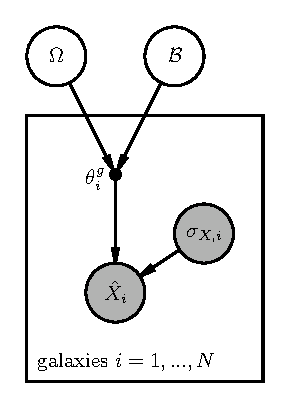
\includegraphics[width=0.6\columnwidth]{figs/graph.pdf}}
    \caption{
        Graphical representation of our hierarchical approach that illustrate
        the relationship among the parameters of our model. 
        Circles are inferred random variables, shaded circles are observed
        quantities, and dots indicate random variables that are deterministic.
        The physical properties of galaxies, $\theta^g_i$, are determined from
        the cosmological and hydrodynamical parameters $\Omega$ and
        $\mathcal{B}$ through the CAMELS-TNG simulation. 
        Then the noisy optical photometry, $\hat{X}_i$, is derived from
        $\theta^g_i$ using SPS and our noise model. 
    }\label{fig:graph}
\end{center}
\vskip -0.2in
\end{figure}

Given this hierarchical model, we can rewrite the posterior as: 
\begin{align}
p(\Omega, \mathcal{B} \given \{{\bfi X_i}\}) 
    =&~\frac{p(\Omega, \mathcal{B})~p(\{{\bfi X_i}\} \given \Omega,
    \mathcal{B})}{p(\{{\bfi X_i}\})}\\
    =&~\frac{p(\Omega, \mathcal{B})}{p(\{\bfi X_i\})}\prod\limits_{i=1}^N 
    p({\bfi X_i}\given \Omega, \mathcal{B})\\
    =&~\frac{p(\Omega, \mathcal{B})}{p(\{\bfi X_i\})}\prod\limits_{i=1}^N 
    \frac{p(\bfi X_i)\,p(\Omega, \mathcal{B}\given{\bfi X_i})}{p(\Omega,
    \mathcal{B})}\\
    %    =&~\frac{p(\Omega, \mathcal{B})}{p(\{{\bfi X_i}\})}\int p(\{{\bfi X_i}\}
    %    \given \{\theta^g_i\})~p(\{\theta^g_i\} \given \Omega, \mathcal{B})~{\rm d}\{\theta^g_i\}.\\
    %    =&~\frac{p(\Omega, \mathcal{B})}{p(\{{\bfi X_i}\})}\prod\limits_{i=1}^N\int
    %    p({\bfi X_i} \given \theta^g_i)~p(\theta^g_i \given \Omega, \mathcal{B})~{\rm d}\theta^g_i\\
    %    =&~\frac{p(\Omega, \mathcal{B})}{p(\{{\bfi X_i}\})}\prod\limits_{i=1}^N\int
    %    \frac{p(\theta^g_i \given {\bfi X_i})~p({\bfi
    %    X_i})}{p(\theta^g_i)}~p(\theta^g_i \given \Omega, \mathcal{B})~{\rm d}\theta^g_i\\
    %    =&~p(\Omega, \mathcal{B})\prod\limits_{i=1}^N\int \frac{~p(\theta^g_i
    %    \given \Omega, \mathcal{B})}{p(\theta^g_i)} p(\theta^g_i \given {\bfi X_i})
    %    ~{\rm d}\theta^g_i\\
    %    =&~p(\Omega, \mathcal{B})\prod\limits_{i=1}^N\int \frac{p(\Omega, \mathcal{B}\given \theta^g_i)}{p(\Omega, \mathcal{B})}
    %p(\theta^g_i \given {\bfi X_i})~{\rm d}\theta^g_i \\
    %     \label{eq:post0}
    %    =&~\frac{1}{p(\Omega, \mathcal{B})^{N-1}}\prod\limits_{i=1}^N\int p(\Omega,
    %    \mathcal{B}\given \theta^g_i) p(\theta^g_i \given {\bfi X_i})~{\rm
    %    d}\theta^g_i  \\
    %     \label{eq:posterior}
    =&~\frac{1}{p(\Omega, \mathcal{B})^{N-1}}\prod\limits_{i=1}^N p(\Omega,
    \mathcal{B}\given {\bfi X_i})\\
\intertext{
    We downsampled the galaxies in the CAMELS-TNG simulations to impose 
    $p(\Omega, \mathcal{B}) = 1$ (Sec.~\ref{sec:sims}), so the posterior
    simply becomes:}
    \label{eq:posterior}
    =&~\prod\limits_{i=1}^N p(\Omega, \mathcal{B}\given {\bfi X_i}).
\end{align} 
Hence, we can evaluate $p(\Omega, \mathcal{B} \given \{{\bfi X_i}\})$, and
sample it, as long as we can accurately estimate $p(\Omega, \mathcal{B}\given
{\bfi X_i})$, the posterior for photometry from an individual galaxy. 

\subsection{Neural Density Estimation} \label{sec:anpe}
One way to accurately estimate $p(\Omega, \mathcal{B}\given {\bfi X_i})$ is
by applying neural density estimation (NDE) to the CAMELS-TNG.
The CAMELS-TNG forward model provides a training dataset of 100,000
parameter-photometry pairs: $\{(\Omega, \mathcal{B}, {\bfi X_i})\}$.
With NDE, we can use this data to train a neural network $q$ with parameters
$\phi$ to estimate 
$p(\Omega, \mathcal{B}\given {\bfi X_i}) \approx
q_\phi(\Omega, \mathcal{B}\given {\bfi X_i})$.
This type of simulaiton-based inference using NDE has now been applied to a
broad range of astronomical applications:
\eg~analyzing gravitational waves~\citep{wong2020, dax2021}, binary
microlensing lensing~\citep{zhang2021}, galaxy SEDs~\cite{hahn2022a}, and
galaxy clustering~\cite{hahn2022d, hahn2023}. 

In this work, our NDE is based on ``normalizing flow'' models~\citep{tabak2010,
tabak2013}, which use neural networks to learn a flexible and bijective
transformation, $f$, that maps a complex target distribution to a simple base
distribution that is fast to evaluate.
$f$ is defined to be invertible and have a tractable Jacobian so that the 
target distribution can be evaluated with change of variables. 
Since $\pi(\bfi{z})$ is easy to evaluate, this enables us to also easily 
evaluate the target distribution.
In our case, the target distribution is 
$p(\Omega, \mathcal{B}\given {\bfi X_i})$ and we set the base distribution to
be a multivariate Gaussian. 
Among different flow architectures, we use Masked Autoregressive
Flow~\citep[MAF;][]{papamakarios2017} models implemented in the $\mathtt{sbi}$
Python
package\footnote{\url{https://github.com/mackelab/sbi/}}~\citep{greenberg2019,
tejero-cantero2020}.

\begin{figure}[ht]
\vskip 0.2in
\begin{center}
    \centerline{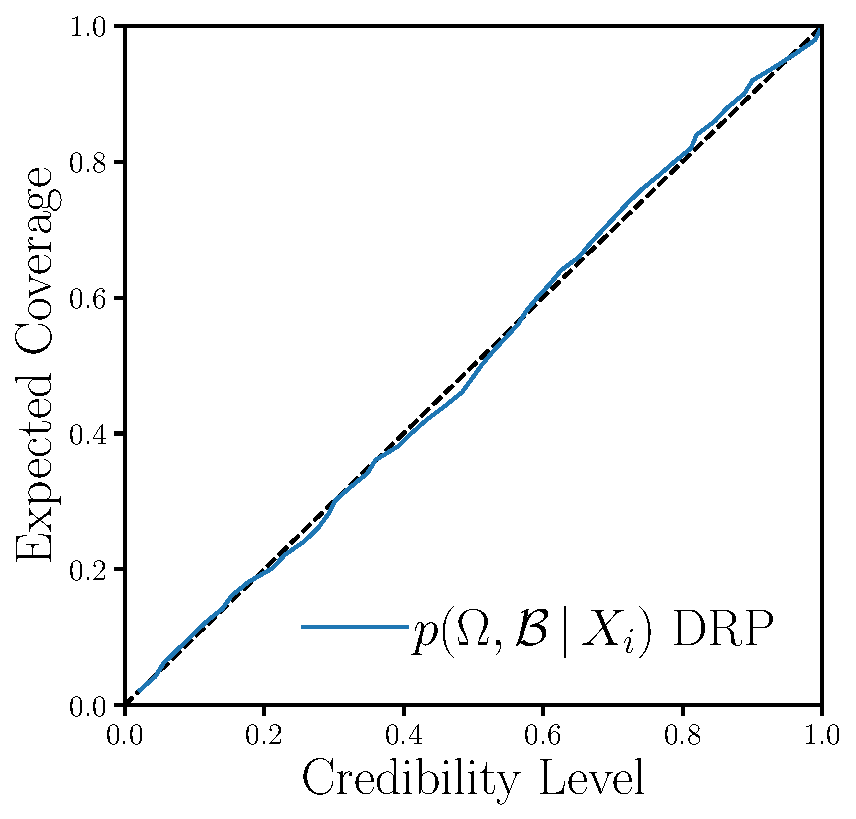
\includegraphics[width=0.6\columnwidth]{figs/tarp_p_omega_x.pdf}}
    \caption{DRP coverage test validating the accuracy of our 
    $q_{\phi}(\Omega, \mathcal{B}\given {\bfi X_i})$ posterior estimate trained
    using the forward modeled CAMELS-TNG data (blue).
    The black-dashed line represents an optimal estimate of the posterior.
    The coverage test demonstrates that $q_\phi$ provides a near optimal
    estimate of the true posterior.
    }\label{fig:tarp}
\end{center}
\vskip -0.2in
\end{figure}

Our goal in training the flow is to determine $q_\phi$ that best approximates 
$p(\Omega, \mathcal{B}\given {\bfi X_i})$. 
We can reformulate this into an optimization problem for determining $\phi$
that minimizes the KL divergence between 
$p(\Omega, \mathcal{B}, {\bfi X_i}) = p(\Omega, \mathcal{B}\given {\bfi X_i})
 p({\bfi X_i})$ and
$q_\phi(\Omega, \mathcal{B}\given {\bfi X_i}) p({\bfi X_i})$.
In practice, we split the $\{(\Omega, \mathcal{B}, {\bfi X_i}\}$ data from
CAMELS-TNG into a training and validation set with a 90/10 split.
Then, we maximize the total log-likelihood 
$\sum_i \log q_{\phi}(\Omega, \mathcal{B}\given {\bfi X_i})$ over the 
training set, which is equivalent to the KL divergence, using the {\sc Adam} 
optimizer~\citep{kingma2017} with a learning rate of $5\times10^{-4}$. 
To prevent overfitting, we evaluate the total log-likelihood on the validation
data at every training epoch and stop the training when the validation 
log-likelihood fails to increase after 20 epochs.  


We determine the architecture of our flow by training a large number of flows
with architectures determined using the \cite{akiba2019} hyperparameter optimization framework.
Afterwards, we define our final flow as an equally weighted ensemble of five
flows with the lowest validation losses: 
$q_{\phi}(\Omega, \mathcal{B}\given {\bfi X_i}) = 
\sum_{j=1}^5 q_{\phi,j}(\Omega, \mathcal{B}\given {\bfi X_i})/5$. 
Ensembling flows with different initializations and architectures improves the
overall robustness of our normalizing flow~\citep{alsing2019}.
To validate the accuracy of $q_\phi$, we use the ``distance to random point''
(DRP) coverage test from \cite{lemos2023}, which is necessary and sufficient to
show that a posterior estimator is optimal. 
In Fig~\ref{fig:tarp}, we present the DRP coverage of $q_\phi$ (blue) and
find that it provides a near optimal estimate of the true posterior.


\begin{figure}[ht]
\vskip 0.2in
\begin{center}
    \centerline{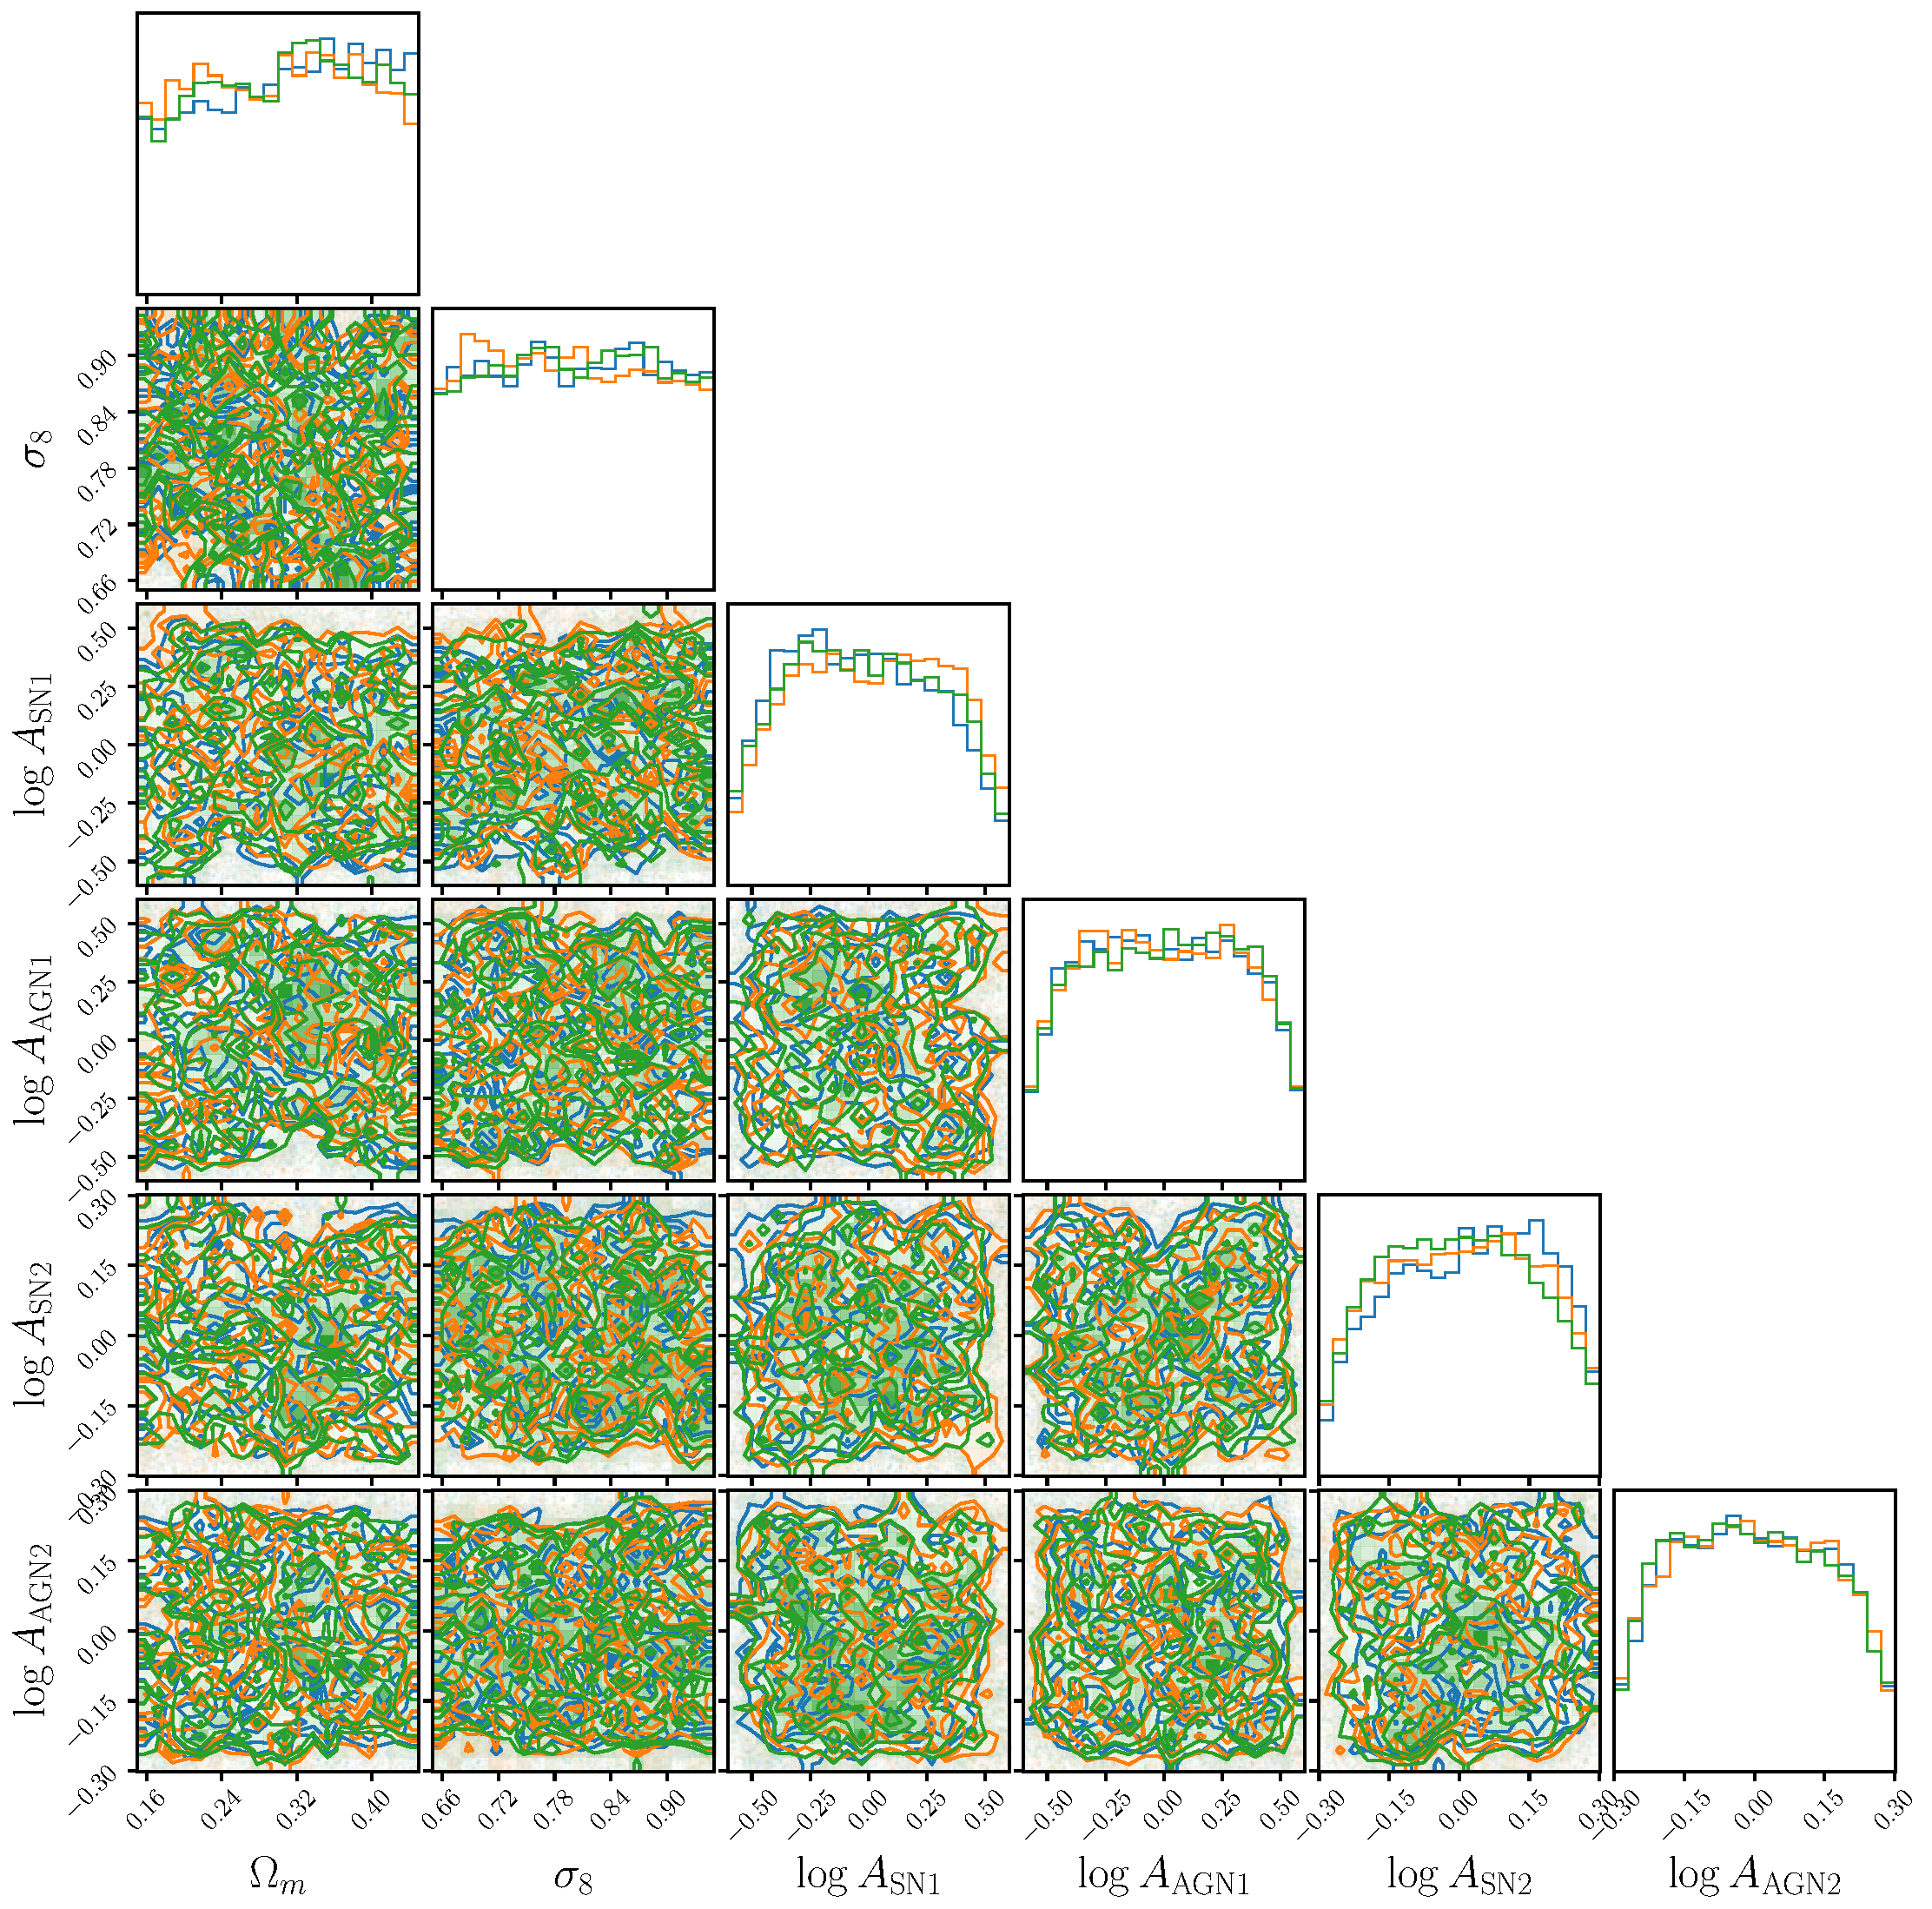
\includegraphics[width=\columnwidth]{figs/p_omega_x_i.pdf}}
    \caption{Estimated posteriors of the cosmological and hydrodynamical 
    parameters ($\Omega$, $mathcal{B}$) from photometry, 
    $q_{\phi}(\Omega, \mathcal{B}\given {\bfi X_i})$,for three arbitrarily 
    selected NSA galaxies. 
    The posteriors correspond to the galaxies marked in Fig.~\ref{fig:nsa}.
    }\label{fig:p_omega_x_i}
\end{center}
\vskip -0.2in
\end{figure}

In Fig.~\ref{fig:p_omega_x_i}, we present 
$q_{\phi}(\Omega, \mathcal{B}\given {\bfi X_i})$
for three arbitrarily selected NSA galaxies. 
The selected galaxies are also marked in Fig.~\ref{fig:nsa}. 
The individual posteriors reveal that  there is very little cosmological
information in the photometry of a single galaxy. 
However, with Eq.~\ref{eq:posterior}, we can extract the cosmological
information from {\em thousands} of galaxies.

% --- results ---  
\section{Results} \label{sec:results}
Our goal in this paper is to infer the posterior of cosmological parameters
$\Omega = \{ \Omega_m, \sigma_8 \}$ and baryonic feedback parameters 
$\mathcal{B} = \{ A_{\rm SN1}, A_{\rm SN2}, A_{\rm AGN1}, A_{\rm AGN2}\}$ from the observed photometry
of galaxies in the NSA catalog, $\{\bfi X_i\}$: 
$p(\Omega, \mathcal{B} \given \{{\bfi X_i}\})$.
We graphically represent our approach in Figure~\ref{fig:graph}.
Circles, shaded circles, and dots represent random variables, observed
quantities, and random variables that are deterministic. 
$\theta_i^g$, the physical properties of galaxies (\emph{e.g.} $M_*$,
star-formation history), are determined from $\Omega$ and $\mathcal{B}$ through
the hydrodynamical models used to construct CAMELS.
Then the photometry $X_i$ is determined from $\theta_i^g$ through the SED model
based on stellar population synthesis (Section~\ref{sec:sim}).  

\begin{figure}
\begin{center}
    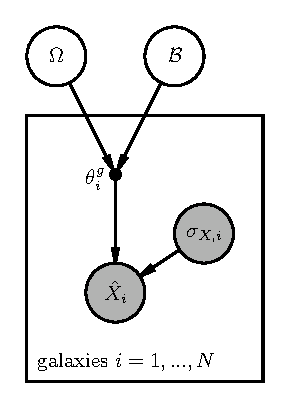
\includegraphics[width=0.4\textwidth]{figs/graph.pdf} 
    \caption{
        Graphical representation of our hierarchical approach that illustrate
        the relationship among the main parameters of our model. 
        Circles are inferred random variables, shaded circles are observed
        quantities, and dots indicate random variables that are deterministic.
    }\label{fig:graph}
\end{center}
\end{figure}


Given this hierarchical model, we can rewrite the posterior of interest: 
\begin{align}
p(\Omega, \mathcal{B} \given \{{\bfi X_i}\}) 
    =&~\frac{p(\Omega, \mathcal{B})~p(\{{\bfi X_i}\} \given \Omega, \mathcal{B})}{p(\{{\bfi X_i}\})}\\
    =&~\frac{p(\Omega, \mathcal{B})}{p(\{{\bfi X_i}\})}\int p(\{{\bfi X_i}\}
    \given \{\theta^g_i\})~p(\{\theta^g_i\} \given \Omega, \mathcal{B})~{\rm d}\{\theta^g_i\}.\\
    =&~\frac{p(\Omega, \mathcal{B})}{p(\{{\bfi X_i}\})}\prod\limits_{i=1}^N\int
    p({\bfi X_i} \given \theta^g_i)~p(\theta^g_i \given \Omega, \mathcal{B})~{\rm d}\theta^g_i\\
    =&~\frac{p(\Omega, \mathcal{B})}{p(\{{\bfi X_i}\})}\prod\limits_{i=1}^N\int
    \frac{p(\theta^g_i \given {\bfi X_i})~p({\bfi
    X_i})}{p(\theta^g_i)}~p(\theta^g_i \given \Omega, \mathcal{B})~{\rm d}\theta^g_i\\
    =&~p(\Omega, \mathcal{B})\prod\limits_{i=1}^N\int \frac{~p(\theta^g_i
    \given \Omega, \mathcal{B})}{p(\theta^g_i)} p(\theta^g_i \given {\bfi X_i})
    ~{\rm d}\theta^g_i\\
    =&~p(\Omega, \mathcal{B})\prod\limits_{i=1}^N\int \frac{p(\Omega, \mathcal{B}\given \theta^g_i)}{p(\Omega, \mathcal{B})}
p(\theta^g_i \given {\bfi X_i})~{\rm d}\theta^g_i \\
     \label{eq:post0}
    =&~\frac{1}{p(\Omega, \mathcal{B})^{N-1}}\prod\limits_{i=1}^N\int p(\Omega,
    \mathcal{B}\given \theta^g_i) p(\theta^g_i \given {\bfi X_i})~{\rm
    d}\theta^g_i  \\
     \label{eq:posterior}
    =&~\frac{1}{p(\Omega, \mathcal{B})^{N-1}}\prod\limits_{i=1}^N p(\Omega,
    \mathcal{B}\given {\bfi X_i}).
\end{align} 
With Eq.~\ref{eq:posterior}

explain that $\theta^g$ are latent variables. 


%\intertext{
%    We estimate the integral using $S_i$ Monte Carlo samples from the
%    individual posteriors $p(\theta^g_i \given {\bfi X_i})$: 
%}
%    \approx&~\frac{1}{p(\Omega, \mathcal{B})^{N-1}}\prod\limits_{i=1}^N\frac{1}{S_i}\sum\limits_{j=1}^{S_i} p(\Omega, \mathcal{B} \given \theta^g_{i,j}).

% --- summary ---  
\input{summary}
\bibliography{goleta}
\bibliographystyle{icml2023}


%%%%%%%%%%%%%%%%%%%%%%%%%%%%%%%%%%%%%%%%%%%%%%%%%%%%%%%%%%%%%%%%%%%%%%%%%%%%%%%
%%%%%%%%%%%%%%%%%%%%%%%%%%%%%%%%%%%%%%%%%%%%%%%%%%%%%%%%%%%%%%%%%%%%%%%%%%%%%%%
% APPENDIX
%%%%%%%%%%%%%%%%%%%%%%%%%%%%%%%%%%%%%%%%%%%%%%%%%%%%%%%%%%%%%%%%%%%%%%%%%%%%%%%
%%%%%%%%%%%%%%%%%%%%%%%%%%%%%%%%%%%%%%%%%%%%%%%%%%%%%%%%%%%%%%%%%%%%%%%%%%%%%%%
\newpage
\appendix
\onecolumn
\section{You \emph{can} have an appendix here.}

You can have as much text here as you want. The main body must be at most $8$ pages long.
For the final version, one more page can be added.
If you want, you can use an appendix like this one, even using the one-column format.
%%%%%%%%%%%%%%%%%%%%%%%%%%%%%%%%%%%%%%%%%%%%%%%%%%%%%%%%%%%%%%%%%%%%%%%%%%%%%%%
%%%%%%%%%%%%%%%%%%%%%%%%%%%%%%%%%%%%%%%%%%%%%%%%%%%%%%%%%%%%%%%%%%%%%%%%%%%%%%%


\end{document}


% This document was modified from the file originally made available by
% Pat Langley and Andrea Danyluk for ICML-2K. This version was created
% by Iain Murray in 2018, and modified by Alexandre Bouchard in
% 2019 and 2021 and by Csaba Szepesvari, Gang Niu and Sivan Sabato in 2022.
% Modified again in 2023 by Sivan Sabato and Jonathan Scarlett.
% Previous contributors include Dan Roy, Lise Getoor and Tobias
% Scheffer, which was slightly modified from the 2010 version by
% Thorsten Joachims & Johannes Fuernkranz, slightly modified from the
% 2009 version by Kiri Wagstaff and Sam Roweis's 2008 version, which is
% slightly modified from Prasad Tadepalli's 2007 version which is a
% lightly changed version of the previous year's version by Andrew
% Moore, which was in turn edited from those of Kristian Kersting and
% Codrina Lauth. Alex Smola contributed to the algorithmic style files.

\section{Electronic Submission}
\label{submission}

Submission to ICML 2023 will be entirely electronic, via a web site
(not email). Information about the submission process and \LaTeX\ templates
are available on the conference web site at:
\begin{center}
\textbf{\texttt{http://icml.cc/}}
\end{center}

The guidelines below will be enforced for initial submissions and
camera-ready copies. Here is a brief summary:
\begin{itemize}
\item Submissions must be in PDF\@. 
\item \textbf{New to this year}: If your paper has appendices, submit the appendix together with the main body and the references \textbf{as a single file}. Reviewers will not look for appendices as a separate PDF file. So if you submit such an extra file, reviewers will very likely miss it.
\item Page limit: The main body of the paper has to be fitted to 8 pages, excluding references and appendices; the space for the latter two is not limited. For the final version of the paper, authors can add one extra page to the main body.
\item \textbf{Do not include author information or acknowledgements} in your
    initial submission.
\item Your paper should be in \textbf{10 point Times font}.
\item Make sure your PDF file only uses Type-1 fonts.
\item Place figure captions \emph{under} the figure (and omit titles from inside
    the graphic file itself). Place table captions \emph{over} the table.
\item References must include page numbers whenever possible and be as complete
    as possible. Place multiple citations in chronological order.
\item Do not alter the style template; in particular, do not compress the paper
    format by reducing the vertical spaces.
\item Keep your abstract brief and self-contained, one paragraph and roughly
    4--6 sentences. Gross violations will require correction at the
    camera-ready phase. The title should have content words capitalized.
\end{itemize}

\subsection{Submitting Papers}

\textbf{Paper Deadline:} The deadline for paper submission that is
advertised on the conference website is strict. If your full,
anonymized, submission does not reach us on time, it will not be
considered for publication. 

\textbf{Anonymous Submission:} ICML uses double-blind review: no identifying
author information may appear on the title page or in the paper
itself. \cref{author info} gives further details.

\textbf{Simultaneous Submission:} ICML will not accept any paper which,
at the time of submission, is under review for another conference or
has already been published. This policy also applies to papers that
overlap substantially in technical content with conference papers
under review or previously published. ICML submissions must not be
submitted to other conferences and journals during ICML's review
period.
%Authors may submit to ICML substantially different versions of journal papers
%that are currently under review by the journal, but not yet accepted
%at the time of submission.
Informal publications, such as technical
reports or papers in workshop proceedings which do not appear in
print, do not fall under these restrictions.

\medskip

Authors must provide their manuscripts in \textbf{PDF} format.
Furthermore, please make sure that files contain only embedded Type-1 fonts
(e.g.,~using the program \texttt{pdffonts} in linux or using
File/DocumentProperties/Fonts in Acrobat). Other fonts (like Type-3)
might come from graphics files imported into the document.

Authors using \textbf{Word} must convert their document to PDF\@. Most
of the latest versions of Word have the facility to do this
automatically. Submissions will not be accepted in Word format or any
format other than PDF\@. Really. We're not joking. Don't send Word.

Those who use \textbf{\LaTeX} should avoid including Type-3 fonts.
Those using \texttt{latex} and \texttt{dvips} may need the following
two commands:

{\footnotesize
\begin{verbatim}
dvips -Ppdf -tletter -G0 -o paper.ps paper.dvi
ps2pdf paper.ps
\end{verbatim}}
It is a zero following the ``-G'', which tells dvips to use
the config.pdf file. Newer \TeX\ distributions don't always need this
option.

Using \texttt{pdflatex} rather than \texttt{latex}, often gives better
results. This program avoids the Type-3 font problem, and supports more
advanced features in the \texttt{microtype} package.

\textbf{Graphics files} should be a reasonable size, and included from
an appropriate format. Use vector formats (.eps/.pdf) for plots,
lossless bitmap formats (.png) for raster graphics with sharp lines, and
jpeg for photo-like images.

The style file uses the \texttt{hyperref} package to make clickable
links in documents. If this causes problems for you, add
\texttt{nohyperref} as one of the options to the \texttt{icml2023}
usepackage statement.


\subsection{Submitting Final Camera-Ready Copy}

The final versions of papers accepted for publication should follow the
same format and naming convention as initial submissions, except that
author information (names and affiliations) should be given. See
\cref{final author} for formatting instructions.

The footnote, ``Preliminary work. Under review by the International
Conference on Machine Learning (ICML). Do not distribute.'' must be
modified to ``\textit{Proceedings of the
$\mathit{40}^{th}$ International Conference on Machine Learning},
Honolulu, Hawaii, USA, PMLR 202, 2023.
Copyright 2023 by the author(s).''

For those using the \textbf{\LaTeX} style file, this change (and others) is
handled automatically by simply changing
$\mathtt{\backslash usepackage\{icml2023\}}$ to
$$\mathtt{\backslash usepackage[accepted]\{icml2023\}}$$
Authors using \textbf{Word} must edit the
footnote on the first page of the document themselves.

Camera-ready copies should have the title of the paper as running head
on each page except the first one. The running title consists of a
single line centered above a horizontal rule which is $1$~point thick.
The running head should be centered, bold and in $9$~point type. The
rule should be $10$~points above the main text. For those using the
\textbf{\LaTeX} style file, the original title is automatically set as running
head using the \texttt{fancyhdr} package which is included in the ICML
2023 style file package. In case that the original title exceeds the
size restrictions, a shorter form can be supplied by using

\verb|\icmltitlerunning{...}|

just before $\mathtt{\backslash begin\{document\}}$.
Authors using \textbf{Word} must edit the header of the document themselves.

\section{Format of the Paper}

All submissions must follow the specified format.

\subsection{Dimensions}




The text of the paper should be formatted in two columns, with an
overall width of 6.75~inches, height of 9.0~inches, and 0.25~inches
between the columns. The left margin should be 0.75~inches and the top
margin 1.0~inch (2.54~cm). The right and bottom margins will depend on
whether you print on US letter or A4 paper, but all final versions
must be produced for US letter size.
Do not write anything on the margins.

The paper body should be set in 10~point type with a vertical spacing
of 11~points. Please use Times typeface throughout the text.

\subsection{Title}

The paper title should be set in 14~point bold type and centered
between two horizontal rules that are 1~point thick, with 1.0~inch
between the top rule and the top edge of the page. Capitalize the
first letter of content words and put the rest of the title in lower
case.

\subsection{Author Information for Submission}
\label{author info}

ICML uses double-blind review, so author information must not appear. If
you are using \LaTeX\/ and the \texttt{icml2023.sty} file, use
\verb+\icmlauthor{...}+ to specify authors and \verb+\icmlaffiliation{...}+ to specify affiliations. (Read the TeX code used to produce this document for an example usage.) The author information
will not be printed unless \texttt{accepted} is passed as an argument to the
style file.
Submissions that include the author information will not
be reviewed.

\subsubsection{Self-Citations}

If you are citing published papers for which you are an author, refer
to yourself in the third person. In particular, do not use phrases
that reveal your identity (e.g., ``in previous work \cite{langley00}, we
have shown \ldots'').

Do not anonymize citations in the reference section. The only exception are manuscripts that are
not yet published (e.g., under submission). If you choose to refer to
such unpublished manuscripts \cite{anonymous}, anonymized copies have
to be submitted
as Supplementary Material via CMT\@. However, keep in mind that an ICML
paper should be self contained and should contain sufficient detail
for the reviewers to evaluate the work. In particular, reviewers are
not required to look at the Supplementary Material when writing their
review (they are not required to look at more than the first $8$ pages of the submitted document).

\subsubsection{Camera-Ready Author Information}
\label{final author}

If a paper is accepted, a final camera-ready copy must be prepared.
%
For camera-ready papers, author information should start 0.3~inches below the
bottom rule surrounding the title. The authors' names should appear in 10~point
bold type, in a row, separated by white space, and centered. Author names should
not be broken across lines. Unbolded superscripted numbers, starting 1, should
be used to refer to affiliations.

Affiliations should be numbered in the order of appearance. A single footnote
block of text should be used to list all the affiliations. (Academic
affiliations should list Department, University, City, State/Region, Country.
Similarly for industrial affiliations.)

Each distinct affiliations should be listed once. If an author has multiple
affiliations, multiple superscripts should be placed after the name, separated
by thin spaces. If the authors would like to highlight equal contribution by
multiple first authors, those authors should have an asterisk placed after their
name in superscript, and the term ``\textsuperscript{*}Equal contribution"
should be placed in the footnote block ahead of the list of affiliations. A
list of corresponding authors and their emails (in the format Full Name
\textless{}email@domain.com\textgreater{}) can follow the list of affiliations.
Ideally only one or two names should be listed.

A sample file with author names is included in the ICML2023 style file
package. Turn on the \texttt{[accepted]} option to the stylefile to
see the names rendered. All of the guidelines above are implemented
by the \LaTeX\ style file.

\subsection{Abstract}

The paper abstract should begin in the left column, 0.4~inches below the final
address. The heading `Abstract' should be centered, bold, and in 11~point type.
The abstract body should use 10~point type, with a vertical spacing of
11~points, and should be indented 0.25~inches more than normal on left-hand and
right-hand margins. Insert 0.4~inches of blank space after the body. Keep your
abstract brief and self-contained, limiting it to one paragraph and roughly 4--6
sentences. Gross violations will require correction at the camera-ready phase.

\subsection{Partitioning the Text}

You should organize your paper into sections and paragraphs to help
readers place a structure on the material and understand its
contributions.

\subsubsection{Sections and Subsections}

Section headings should be numbered, flush left, and set in 11~pt bold
type with the content words capitalized. Leave 0.25~inches of space
before the heading and 0.15~inches after the heading.

Similarly, subsection headings should be numbered, flush left, and set
in 10~pt bold type with the content words capitalized. Leave
0.2~inches of space before the heading and 0.13~inches afterward.

Finally, subsubsection headings should be numbered, flush left, and
set in 10~pt small caps with the content words capitalized. Leave
0.18~inches of space before the heading and 0.1~inches after the
heading.

Please use no more than three levels of headings.

\subsubsection{Paragraphs and Footnotes}

Within each section or subsection, you should further partition the
paper into paragraphs. Do not indent the first line of a given
paragraph, but insert a blank line between succeeding ones.

You can use footnotes\footnote{Footnotes
should be complete sentences.} to provide readers with additional
information about a topic without interrupting the flow of the paper.
Indicate footnotes with a number in the text where the point is most
relevant. Place the footnote in 9~point type at the bottom of the
column in which it appears. Precede the first footnote in a column
with a horizontal rule of 0.8~inches.\footnote{Multiple footnotes can
appear in each column, in the same order as they appear in the text,
but spread them across columns and pages if possible.}

\begin{figure}[ht]
\vskip 0.2in
\begin{center}
\centerline{\includegraphics[width=\columnwidth]{icml_numpapers}}
\caption{Historical locations and number of accepted papers for International
Machine Learning Conferences (ICML 1993 -- ICML 2008) and International
Workshops on Machine Learning (ML 1988 -- ML 1992). At the time this figure was
produced, the number of accepted papers for ICML 2008 was unknown and instead
estimated.}
\label{icml-historical}
\end{center}
\vskip -0.2in
\end{figure}

\subsection{Figures}

You may want to include figures in the paper to illustrate
your approach and results. Such artwork should be centered,
legible, and separated from the text. Lines should be dark and at
least 0.5~points thick for purposes of reproduction, and text should
not appear on a gray background.

Label all distinct components of each figure. If the figure takes the
form of a graph, then give a name for each axis and include a legend
that briefly describes each curve. Do not include a title inside the
figure; instead, the caption should serve this function.

Number figures sequentially, placing the figure number and caption
\emph{after} the graphics, with at least 0.1~inches of space before
the caption and 0.1~inches after it, as in
\cref{icml-historical}. The figure caption should be set in
9~point type and centered unless it runs two or more lines, in which
case it should be flush left. You may float figures to the top or
bottom of a column, and you may set wide figures across both columns
(use the environment \texttt{figure*} in \LaTeX). Always place
two-column figures at the top or bottom of the page.

\subsection{Algorithms}

If you are using \LaTeX, please use the ``algorithm'' and ``algorithmic''
environments to format pseudocode. These require
the corresponding stylefiles, algorithm.sty and
algorithmic.sty, which are supplied with this package.
\cref{alg:example} shows an example.

\begin{algorithm}[tb]
   \caption{Bubble Sort}
   \label{alg:example}
\begin{algorithmic}
   \STATE {\bfseries Input:} data $x_i$, size $m$
   \REPEAT
   \STATE Initialize $noChange = true$.
   \FOR{$i=1$ {\bfseries to} $m-1$}
   \IF{$x_i > x_{i+1}$}
   \STATE Swap $x_i$ and $x_{i+1}$
   \STATE $noChange = false$
   \ENDIF
   \ENDFOR
   \UNTIL{$noChange$ is $true$}
\end{algorithmic}
\end{algorithm}

\subsection{Tables}

You may also want to include tables that summarize material. Like
figures, these should be centered, legible, and numbered consecutively.
However, place the title \emph{above} the table with at least
0.1~inches of space before the title and the same after it, as in
\cref{sample-table}. The table title should be set in 9~point
type and centered unless it runs two or more lines, in which case it
should be flush left.

% Note use of \abovespace and \belowspace to get reasonable spacing
% above and below tabular lines.

\begin{table}[t]
\caption{Classification accuracies for naive Bayes and flexible
Bayes on various data sets.}
\label{sample-table}
\vskip 0.15in
\begin{center}
\begin{small}
\begin{sc}
\begin{tabular}{lcccr}
\toprule
Data set & Naive & Flexible & Better? \\
\midrule
Breast    & 95.9$\pm$ 0.2& 96.7$\pm$ 0.2& $\surd$ \\
Cleveland & 83.3$\pm$ 0.6& 80.0$\pm$ 0.6& $\times$\\
Glass2    & 61.9$\pm$ 1.4& 83.8$\pm$ 0.7& $\surd$ \\
Credit    & 74.8$\pm$ 0.5& 78.3$\pm$ 0.6&         \\
Horse     & 73.3$\pm$ 0.9& 69.7$\pm$ 1.0& $\times$\\
Meta      & 67.1$\pm$ 0.6& 76.5$\pm$ 0.5& $\surd$ \\
Pima      & 75.1$\pm$ 0.6& 73.9$\pm$ 0.5&         \\
Vehicle   & 44.9$\pm$ 0.6& 61.5$\pm$ 0.4& $\surd$ \\
\bottomrule
\end{tabular}
\end{sc}
\end{small}
\end{center}
\vskip -0.1in
\end{table}

Tables contain textual material, whereas figures contain graphical material.
Specify the contents of each row and column in the table's topmost
row. Again, you may float tables to a column's top or bottom, and set
wide tables across both columns. Place two-column tables at the
top or bottom of the page.

\subsection{Theorems and such}
The preferred way is to number definitions, propositions, lemmas, etc. consecutively, within sections, as shown below.
\begin{definition}
\label{def:inj}
A function $f:X \to Y$ is injective if for any $x,y\in X$ different, $f(x)\ne f(y)$.
\end{definition}
Using \cref{def:inj} we immediate get the following result:
\begin{proposition}
If $f$ is injective mapping a set $X$ to another set $Y$, 
the cardinality of $Y$ is at least as large as that of $X$
\end{proposition}
\begin{proof} 
Left as an exercise to the reader. 
\end{proof}
\cref{lem:usefullemma} stated next will prove to be useful.
\begin{lemma}
\label{lem:usefullemma}
For any $f:X \to Y$ and $g:Y\to Z$ injective functions, $f \circ g$ is injective.
\end{lemma}
\begin{theorem}
\label{thm:bigtheorem}
If $f:X\to Y$ is bijective, the cardinality of $X$ and $Y$ are the same.
\end{theorem}
An easy corollary of \cref{thm:bigtheorem} is the following:
\begin{corollary}
If $f:X\to Y$ is bijective, 
the cardinality of $X$ is at least as large as that of $Y$.
\end{corollary}
\begin{assumption}
The set $X$ is finite.
\label{ass:xfinite}
\end{assumption}
\begin{remark}
According to some, it is only the finite case (cf. \cref{ass:xfinite}) that is interesting.
\end{remark}
%restatable

\subsection{Citations and References}

Please use APA reference format regardless of your formatter
or word processor. If you rely on the \LaTeX\/ bibliographic
facility, use \texttt{natbib.sty} and \texttt{icml2023.bst}
included in the style-file package to obtain this format.

Citations within the text should include the authors' last names and
year. If the authors' names are included in the sentence, place only
the year in parentheses, for example when referencing Arthur Samuel's
pioneering work \yrcite{Samuel59}. Otherwise place the entire
reference in parentheses with the authors and year separated by a
comma \cite{Samuel59}. List multiple references separated by
semicolons \cite{kearns89,Samuel59,mitchell80}. Use the `et~al.'
construct only for citations with three or more authors or after
listing all authors to a publication in an earlier reference \cite{MachineLearningI}.

Authors should cite their own work in the third person
in the initial version of their paper submitted for blind review.
Please refer to \cref{author info} for detailed instructions on how to
cite your own papers.

Use an unnumbered first-level section heading for the references, and use a
hanging indent style, with the first line of the reference flush against the
left margin and subsequent lines indented by 10 points. The references at the
end of this document give examples for journal articles \cite{Samuel59},
conference publications \cite{langley00}, book chapters \cite{Newell81}, books
\cite{DudaHart2nd}, edited volumes \cite{MachineLearningI}, technical reports
\cite{mitchell80}, and dissertations \cite{kearns89}.

Alphabetize references by the surnames of the first authors, with
single author entries preceding multiple author entries. Order
references for the same authors by year of publication, with the
earliest first. Make sure that each reference includes all relevant
information (e.g., page numbers).

Please put some effort into making references complete, presentable, and
consistent, e.g. use the actual current name of authors.
If using bibtex, please protect capital letters of names and
abbreviations in titles, for example, use \{B\}ayesian or \{L\}ipschitz
in your .bib file.

\section*{Accessibility}
Authors are kindly asked to make their submissions as accessible as possible for everyone including people with disabilities and sensory or neurological differences.
Tips of how to achieve this and what to pay attention to will be provided on the conference website \url{http://icml.cc/}.

\section*{Software and Data}

If a paper is accepted, we strongly encourage the publication of software and data with the
camera-ready version of the paper whenever appropriate. This can be
done by including a URL in the camera-ready copy. However, \textbf{do not}
include URLs that reveal your institution or identity in your
submission for review. Instead, provide an anonymous URL or upload
the material as ``Supplementary Material'' into the CMT reviewing
system. Note that reviewers are not required to look at this material
when writing their review.

% Acknowledgements should only appear in the accepted version.
\section*{Acknowledgements}

\textbf{Do not} include acknowledgements in the initial version of
the paper submitted for blind review.

If a paper is accepted, the final camera-ready version can (and
probably should) include acknowledgements. In this case, please
place such acknowledgements in an unnumbered section at the
end of the paper. Typically, this will include thanks to reviewers
who gave useful comments, to colleagues who contributed to the ideas,
and to funding agencies and corporate sponsors that provided financial
support.


% In the unusual situation where you want a paper to appear in the
% references without citing it in the main text, use \nocite
\nocite{langley00}

